% ============================================================
%  Příprava na maturitu – Elektrotechnika
%  Okruh 13: Integrované obvody a desky plošných spojů
% ============================================================

\documentclass[a4paper,10pt]{article}

\usepackage[T1]{fontenc}
\usepackage[utf8]{inputenc}
\usepackage[left=2.0cm, right=1.8cm, top=1.8cm, bottom=1.8cm]{geometry}
\usepackage{parskip}
\usepackage{xcolor}
\usepackage{tabularx}
\usepackage{booktabs}
\usepackage{tikz}
\usepackage{mdframed}
\usepackage{amsmath}
\usepackage{enumitem}

\usetikzlibrary{arrows.meta, positioning, decorations.pathmorphing, shapes.geometric, calc, patterns}

% --- Barvy ---
\definecolor{accent}{HTML}{1A3A5C}
\definecolor{lightblue}{HTML}{EAF2F8}
\definecolor{lightyellow}{HTML}{FDFBE4}
\definecolor{lightgreen}{HTML}{EAF7EA}
\definecolor{lightred}{HTML}{FDE8E8}
\definecolor{lightgray}{HTML}{F4F4F4}
\definecolor{pcbgreen}{HTML}{2E8B57}
\definecolor{copper}{HTML}{B87333}

% --- Boxy ---
\newmdenv[backgroundcolor=lightblue,linecolor=accent!40,roundcorner=4pt,
  innertopmargin=6pt,innerbottommargin=6pt,innerleftmargin=8pt,innerrightmargin=8pt]{pojmybox}
\newmdenv[backgroundcolor=lightyellow,linecolor=accent!30,roundcorner=4pt,
  innertopmargin=6pt,innerbottommargin=6pt,innerleftmargin=8pt,innerrightmargin=8pt]{vysvetlenibox}
\newmdenv[backgroundcolor=lightgreen,linecolor=accent!40,roundcorner=4pt,
  innertopmargin=6pt,innerbottommargin=6pt,innerleftmargin=8pt,innerrightmargin=8pt]{vzorcebox}
\newmdenv[backgroundcolor=lightred,linecolor=accent!30,roundcorner=4pt,
  innertopmargin=6pt,innerbottommargin=6pt,innerleftmargin=8pt,innerrightmargin=8pt]{durazbox}

\setlist[itemize]{noitemsep, leftmargin=1.4em, topsep=2pt}
\setlist[enumerate]{noitemsep, leftmargin=1.4em, topsep=2pt}

% --- Zkratka pro jednotky ---
\newcommand{\jednotka}[1]{\,[\mathrm{#1}]}

\begin{document}

% ============================================================
\section*{\large Okruh 13 – Integrované obvody a desky plošných spojů}

\begin{pojmybox}
\textbf{Klíčové pojmy:}
integrovaný obvod (IO), monolitický IO, hustota integrace, Moorův zákon, analogový/číslicový obvod, pouzdra (DIP, SOIC, QFP, BGA), deska plošných spojů (DPS/PCB), materiál FR-4, měděná fólie, fotolitografie, leptání, nepájivá maska, prokovený otvor (via)
\end{pojmybox}

\begin{vysvetlenibox}

% ================================================================
\subsection*{1. Integrované obvody (IO / IC)}

Integrovaný obvod je elektronická součástka, která v jednom pouzdře spojuje (integruje) obrovské množství základních prvků (tranzistorů, diod, rezistorů). Jsou vytvořeny na jediném krystalu polovodiče (nejčastěji křemíku) – proto se jim říká **monolitické** IO.

\textbf{Výhody IO proti diskrétním součástkám:}
Obrovská miniaturizace, extrémní spolehlivost (odpadají tisíce mechanických pájených spojů), zanedbatelná spotřeba, vysoká rychlost a velmi nízká cena za jeden logický prvek (tranzistor).

\begin{durazbox}
\textbf{Moorův zákon (1965):} Gordon Moore (spoluzakladatel Intelu) vyslovil empirické pravidlo, že **počet tranzistorů v integrovaném obvodu se zdvojnásobí přibližně každé dva roky** při zachování stejné ceny. (Dnes už narážíme na fyzikální limity velikosti atomů křemíku).
\end{durazbox}

\textbf{Rozdělení podle zpracovávaného signálu:}
\begin{itemize}
    \item \textbf{Analogové (Lineární):} Zpracovávají spojitý signál (Operační zesilovače, stabilizátory napětí, nf zesilovače).
    \item \textbf{Číslicové (Digitální):} Pracují pouze se stavy 0 a 1 (Mikroprocesory, paměti RAM, logická hradla).
    \item \textbf{Smíšené:} Obsahují obojí (A/D a D/A převodníky).
\end{itemize}

% ================================================================
\subsection*{2. Pouzdra integrovaných obvodů}

Křemíkový čip je velmi křehký, proto se zalévá do plastového nebo keramického pouzdra, které má vyvedené piny pro připájení k desce.

\begin{center}
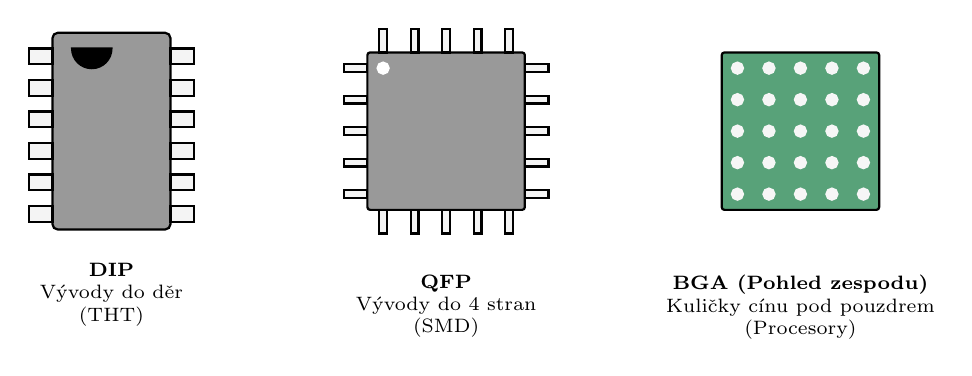
\begin{tikzpicture}[>=Stealth, font=\scriptsize, thick]
  % DIP
  \begin{scope}[xshift=0cm]
    \draw[fill=gray!80, rounded corners=2pt] (0,0) rectangle (1.5, 2.5);
    \filldraw[black] (0.75, 2.3) arc (0:-180:0.25) -- cycle; % Značka pinu 1
    \foreach \y in {0.2, 0.6, 1.0, 1.4, 1.8, 2.2} {
      \draw[fill=lightgray] (-0.3, \y-0.1) rectangle (0, \y+0.1);
      \draw[fill=lightgray] (1.5, \y-0.1) rectangle (1.8, \y+0.1);
    }
    \node[align=center, below] at (0.75, -0.3) {\textbf{DIP}\\Vývody do děr\\(THT)};
  \end{scope}

  % QFP
  \begin{scope}[xshift=4cm, yshift=0.25cm]
    \draw[fill=gray!80, rounded corners=1pt] (0,0) rectangle (2, 2);
    \filldraw[white] (0.2, 1.8) circle (2pt); % Značka pinu 1
    \foreach \x in {0.2, 0.6, 1.0, 1.4, 1.8} {
      \draw[fill=lightgray] (\x-0.05, 2) rectangle (\x+0.05, 2.3);
      \draw[fill=lightgray] (\x-0.05, 0) rectangle (\x+0.05, -0.3);
      \draw[fill=lightgray] (-0.3, \x-0.05) rectangle (0, \x+0.05);
      \draw[fill=lightgray] (2, \x-0.05) rectangle (2.3, \x+0.05);
    }
    \node[align=center, below] at (1, -0.7) {\textbf{QFP}\\Vývody do 4 stran\\(SMD)};
  \end{scope}
  
  % BGA
  \begin{scope}[xshift=8.5cm, yshift=0.25cm]
    \draw[fill=pcbgreen!80, rounded corners=1pt] (0,0) rectangle (2, 2);
    \foreach \x in {0.2, 0.6, 1.0, 1.4, 1.8} {
      \foreach \y in {0.2, 0.6, 1.0, 1.4, 1.8} {
        \filldraw[lightgray!80!white] (\x, \y) circle (2pt);
      }
    }
    \node[align=center, below] at (1, -0.7) {\textbf{BGA (Pohled zespodu)}\\Kuličky cínu pod pouzdrem\\(Procesory)};
  \end{scope}
\end{tikzpicture}
\end{center}

% ================================================================
\subsection*{3. Desky plošných spojů (DPS / PCB)}

Deska plošných spojů (Printed Circuit Board) plní dvě základní funkce: **mechanicky nese** součástky a **elektricky je propojuje** pomocí měděných cest, takže odpadá propojování změti drátů.

\textbf{Základní materiál:} Nejpoužívanějším materiálem je \textbf{FR-4} (žáruvzdorný sklotextit pojený epoxidovou pryskyřicí). Ten je z jedné nebo obou stran potažen tenkou vrstvou čisté mědi (obvykle o tloušťce $35\,\mu\mathrm{m}$).

\begin{center}
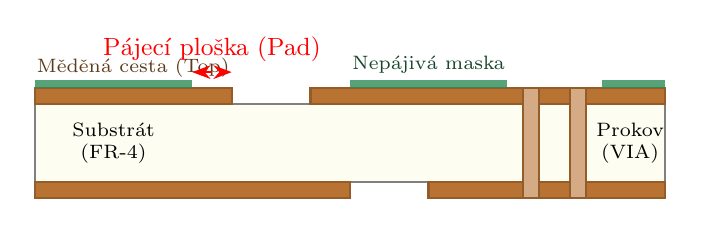
\begin{tikzpicture}[>=Stealth, font=\small, thick]
  % Jádro FR4
  \draw[fill=lightyellow!50, draw=gray] (0, 1) rectangle (8, 2);
  \node[font=\scriptsize, align=center] at (1, 1.5) {Substrát\\(FR-4)};

  % Měděné vrstvy (Copper)
  \draw[fill=copper, draw=copper!80!black] (0, 2) rectangle (2.5, 2.2);
  \draw[fill=copper, draw=copper!80!black] (3.5, 2) rectangle (8, 2.2);
  \draw[fill=copper, draw=copper!80!black] (0, 0.8) rectangle (4, 1);
  \draw[fill=copper, draw=copper!80!black] (5, 0.8) rectangle (8, 1);
  
  \node[font=\scriptsize, align=center, text=copper!50!black, above] at (1.25, 2.2) {Měděná cesta (Top)};

  % Prokov (Via)
  \draw[fill=copper!60, draw=copper!80!black] (6.2, 0.8) rectangle (6.4, 2.2);
  \draw[fill=copper!60, draw=copper!80!black] (6.8, 0.8) rectangle (7.0, 2.2);
  \node[font=\scriptsize, align=center, right] at (7.0, 1.5) {Prokov\\(VIA)};

  % Nepájivá maska (Soldermask)
  \draw[fill=pcbgreen, opacity=0.8, draw=none] (0, 2.2) rectangle (2, 2.3);
  \draw[fill=pcbgreen, opacity=0.8, draw=none] (4, 2.2) rectangle (6, 2.3);
  \draw[fill=pcbgreen, opacity=0.8, draw=none] (7.2, 2.2) rectangle (8, 2.3);
  
  \node[font=\scriptsize, pcbgreen!50!black] at (5, 2.5) {Nepájivá maska};
  
  % SMD Pad (Pájecí ploška bez masky)
  \draw[<->, dashed, red] (2, 2.4) -- (2.5, 2.4) node[midway, above] {Pájecí ploška (Pad)};
\end{tikzpicture}
\end{center}

\textbf{Vrstvy moderní DPS:}
\begin{enumerate}
    \item \textbf{Vodivé cesty (Měď):} Propojují součástky. K propojení horní a spodní vrstvy slouží \textbf{prokovy (vias)} – vyvrtané a zevnitř galvanicky poměděné otvory.
    \item \textbf{Nepájivá maska (Soldermask):} Typicky zelený (nebo modrý, černý) lak. Zabraňuje oxidaci mědi, chrání před zkraty a zabraňuje rozlití cínu při pájení mimo pájecí plošky (pady).
    \item \textbf{Potisk (Silkscreen):} Bílá barva, obsahuje obrysy součástek, jejich označení (např. R1, C4, U2) a hodnoty pro usnadnění osazování a oprav.
\end{enumerate}

% ================================================================
\subsection*{4. Výroba DPS (Subtraktivní metoda / Leptání)}

Jak vyrobit ze souvislé měděné fólie jednotlivé oddělené cestičky? Proces využívá \textbf{fotolitografii}:

\begin{enumerate}
    \item \textbf{Návrh:} V počítači (CAD softwary jako Eagle, KiCad, Altium) se nakreslí schéma a následně se součástky rozloží na desku a program vygeneruje cestičky. Výstupem jsou tzv. \textbf{Gerber data}.
    \item \textbf{Příprava desky:} Na celoměděnou desku se nanese vrstva \textbf{fotorezistu} (látka citlivá na UV světlo).
    \item \textbf{Osvit:} Na desku se přiloží film s vytištěným motivem cestiček a ozáří se UV světlem. Kde je film průhledný, tam fotorezist vytvrdne. Kde je film černý, fotorezist zůstane měkký.
    \item \textbf{Vyvolání:} Deska se vloží do vývojky (např. NaOH), která smyje měkký (neozářený) fotorezist. Zůstane jen tvrdý fotorezist přesně ve tvaru budoucích cestiček.
    \item \textbf{Leptání (Subtrakce):} Deska se ponoří do leptacího roztoku (např. chlorid železitý $\mathrm{FeCl_3}$ nebo směs $\mathrm{HCl} + \mathrm{H_2O_2}$). Leptadlo "sežere" veškerou holou měď. Měď schovaná pod vytvrzeným fotorezistem je uchráněna.
    \item \textbf{Dokončení:} Odstraní se zbytky fotorezistu, vyvrtají se díry, nanesou se prokovy, nepájivá maska a deska je připravena k osazení (připájení) součástek.
\end{enumerate}

% ================================================================
\subsection*{5. Typy DPS podle počtu vrstev}

\begin{itemize}
    \item \textbf{Jednovrstvé:} Měď je jen z jedné strany. Nejlevnější (levná elektronika, napájecí zdroje). Nelze křížit cesty bez drátových propojek.
    \item \textbf{Dvouvrstvé:} Měď nahoře (Top) i dole (Bottom), spojená prokovy. Dnes naprostý standard pro běžné obvody.
    \item \textbf{Vícevrstvé (Multilayer):} Obsahují vnitřní měděné vrstvy (např. 4, 6, 8 vrstev). Vyrábí se slepením tenčích dvouvrstvých desek pomocí izolačních fólií (prepreg) za tepla a tlaku. \textbf{Využití:} Základní desky PC, grafické karty, telefony. Vnitřní vrstvy slouží často jako rozvod napájení (VCC) a zemnící roviny (GND) pro dokonalé odstínění rušení u vysokofrekvenčních a rychlých číslicových obvodů.
\end{itemize}

\end{vysvetlenibox}

\end{document}